\documentclass[12pt, a4paper]{article}
 
% Russian-specific packages
%--------------------------------------
\usepackage[T2A]{fontenc}
\usepackage[utf8]{inputenc}
\usepackage[russian]{babel}
%--------------------------------------

% Extra packages
%--------------------------------------
\usepackage{xcolor}
\usepackage{mathtools}
\usepackage{mathcmd}
\usepackage{cmap}
\usepackage{graphicx}
\graphicspath{{./images/}{./progs/pdf/}}
\usepackage[width=150mm, top=25mm, bottom=25mm]{geometry}
\everymath{\displaystyle}
%--------------------------------------

\begin{document}
	\begin{titlepage}
	\begin{center}
		\Huge
		\textbf{Практикум на ЭВМ}
		\vspace{0.5cm}
		
		\Large
		Аппроксимация задачи с помощью метода конечных элементов
		\vspace{1.5cm}
		
		\LARGE
		\textbf{Прокашев Максим Павлович}
		
		\vspace{0.5cm}
		\textbf{411 группа}
		
		\vspace{0.5cm}
		\today
		
		\vfill
		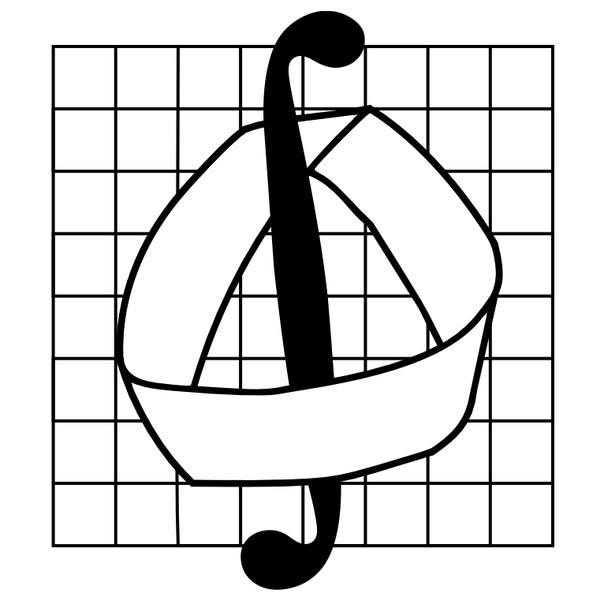
\includegraphics[width=6cm]{math_logo}
		\vspace{0.5cm}
		
		\Large
		2021
	\end{center}
\end{titlepage}
	
	\section{Условие задачи}
	\vspace{0.5cm}
	\begin{equation*}
		\begin{cases}
			\int_{0}^{1}  x^2 + u^2 dt \to \inf \\
			x(0) = 1 \\
			\ddot{x} + \sqrt{2} x e^{-\alpha t} = u
   		\end{cases}
 	\end{equation*}
	$$
		\alpha = \{ 0.0,\ 0.01,\ 1.0,\ 10.0 \}
	$$
	
	\section{Формализация задачи}
	\vspace{0.5cm}
	Предположим, что $x_1(t) = x(t)$ и $x_2(t) = \dot{x_1}(t) = \dot{x}(t)$. \\
	Тогда система имеет вид: \\
	\begin{equation*}
		\begin{cases}
			\int_{0}^{1}  x_1^2 + u^2 dt \to \inf \\
			x_1(0) = 1 \\
			\dot{x}_2 + \sqrt{2} x_1 e^{-\alpha t} = u \\
			\dot{x_1}(t) = x_2(t)
   		\end{cases}
 	\end{equation*} \\
 	Выпишем \textbf{Лагранжиан}: \\
 	\begin{align*}
 		&L = p_1(\dot{x}_1 - x_2) + p_2(\dot{x}_2 - u + \sqrt{2} x_1 e^{-\alpha t})
 			+ \lambda_0(x_1^2 + u^2) \\
 		&l = \lambda_1(x_1(0) - 1)
 	\end{align*} \\
 	Уравнение \textbf{Эйлера-Лагранжа} $\frac{d}{dt} L_{\dot{x}_i} = L_{x_i}$: \\
 	\begin{equation*}
		\begin{cases}
			\frac{d}{dt} p_1 = \sqrt{2} p_2 e^{-\alpha t} + 2 \lambda_0 x_1 \\\\
			\frac{d}{dt} p_2 = -p_1
   		\end{cases}
 	\end{equation*} \\
 	Условия \textbf{Трансверсиальности} $L_{\dot{x}_i}(t_j) = (-1)^j l_{x_i(t_j)}$: \\
 	\begin{equation*}
		\begin{cases}
			p_1(0) = \lambda_1 \\
			p_1(1) = 0 \\
			p_2(0) = 0 \\
			p_2(1) = 0 \\
   		\end{cases}
 	\end{equation*} \\
 	Условие \textbf{Оптимальности}:
 	\begin{equation*}
		\hat{u} = argmin(-p_2 u + \lambda_0 u^2)
 	\end{equation*} \\
 	Если $\lambda_0 = 0$, то: 
 	\begin{align*}
 		&p_2 = 0 \Rightarrow p_1 = 0 \Rightarrow \lambda_1 = 0 \Rightarrow neron \\
 		&p_2 \neq 0 \Rightarrow u \ - \ is\ not \ limited
 	\end{align*} \\
 	Тогда, пусть $\lambda_0 = 1$, тогда $\hat{u} = argmin(u^2 - p_2 u)$, 
 	и минимум этой параболы достигается при $\hat{u} = \frac{p_2}{2}$ \\
 	В итоге, получаем краевую задачу: \\
 	\begin{equation*}
		\begin{cases}
			\dot{x}_1 = x_2 \\
			\dot{x}_2 = \frac{p_2}{2} - \sqrt{2} x_1 e^{-\alpha t} \\
			\dot{p}_1 = 2 x_1 + \sqrt{2} p_2 e^{-\alpha t} \\
			\dot{p}_2 = -p_1 \\
			x_1(0) = 1 \\
			p_1(1) = 0 \\
			p_2(0) = 0 \\
			p_2(1) = 0
   		\end{cases}
 	\end{equation*} \\
 	
 	\section{Результаты}
	\vspace{0.5cm}
	\begin{table}[h!]
	\centering
 		\begin{tabular}{||c c c c c c||} 
 			\hline
 			$\alpha$ & Step & $x_2(0)$ & $p_1(0)$ & min & norm \\ [0.5ex] 
 			\hline
 			\hline
 			0.0 & 4 & -1.2256528222525 & -8.4810303829262 & 0.274772855 & 1.24737678e-15 \\ 
 			0.01 & 3 & -1.2259616030500 & -8.4716882860246 & 0.274705890 & 5.18680126e-15 \\
 			0.5 & 3 & -1.2413207753833 & -8.0757291823282 & 0.271650811 & 2.06187941e-15 \\
 			1 & 3 & -1.2568427330660 & -7.7712687231997 & 0.268964556 & 5.26506416e-15 \\
 			5 & 3 & -1.3481839099619 & -6.8304079309184 & 0.257446938 & 1.77067326e-15 \\
 			10 & 3 & -1.4026857970956 & -6.6019584824634 & 0.252993172 & 5.40779574e-16 \\ [1ex] 
 			\hline
 		\end{tabular}
	\end{table}
\end{document} 












